\chapter{\label{sec:modelling_SB}Modellierung von Strukturbatterien}
Die Modellierung von Strukturbatterien auf der Mirkoskalenebene wurde in den letzten Jahren maßgeblich durch die Arbeiten von Carlstedt~\cite{Carlstedt2018,Carlstedt2019,Carlstedt2022a,Carlstedt2023} vorrangetrieben. Modelle und die Kopplung der mechansichen, elektrochemischen und thermischen Effekte wurde bereits erbracht~\cite{Carlstedt2022,Carlstedt2022b}. Des Weiteren sind aus der Forschung zu herkömmlichen Batterien auch noch andere Ansätze bekannt, die in Kaptiel~\ref{sec:existing_micro_models} kurz erläutert werden sollen. Die Modelle von Carlstedt beschreiben, allerdings vorranging das Verhalten auf der Mikro- oder Partikelebene. Jedoch existiert eine Vielzahl an Arbeiten, die gezeigt haben, wie für konventionelle Batterien eine mittels Homogenisierung, diese Modelle für höhere Skalen adaptiert werden können. Mit Hilfe dieser Methoden wird in Kapitel~\ref{sec:homogenisation} die Modellierung für die Makroebene hergeleitet.

\section{\label{sec:existing_micro_models}Bestehende Mikroskalen Modellierungen}

Die auf der Mirko- oder Partikelebene stattfindenden Prozesse sind unabhängig davon, ob eine konventionelle oder eine Strukturbatterie modelliert wird. Einige Prozesse spielen allerdings für konventionelle Batterien nur eine untergeordente Rolle, weshalb diese oft ignoriert oder vereinfacht werden~\cite{Carlstedt2020a}. Der Ionentransport ist dabei der wichtigste Prozess~\cite{Carlstedt2019b}. Dabei bestehen nach \textsc{Newman} wesentliche Unterschide zwischen flüssige und festen Phasen~\cite{Newman2021}. Da sowohl  konventionelle Batterien, als auch Strukturbatterien, mit zweiphasigen Elektrolyten einen Ionentransport durch beide Phasen besitz lassen sich kann ihr Verhalten in erster Näherung durch die folgenden fünf Differnetialgleichungen\footnote{auch unter dem Namen \textsc{Doyle}-\textsc{Fuller}-\textsc{Newman}-Modell bekannt} beschrieben werden~\cite{Plett2015}.
\begin{enumerate}
    \item Ladungserhalt in homogenen Festkörpern
    \begin{equation}
        \nabla \cdot \boldsymbol{i}_{\text{s}} = \nabla \cdot \left( - \sigma \cdot \nabla \phi_{\text{s}} \right) = 0
    \end{equation}

    \item Massenserhalt in homogenen Festkörpern
    \begin{equation}
        \frac{\partial c_{\text{s}}}{\partial t}  = \nabla \cdot \left( D_{\text{s}} \nabla c_{\text{s}} \right) = 0
    \end{equation}

    \item Massenerhalt in dem homogenen Elektrolyt
    \begin{equation}
        \frac{\partial c_e}{\partial t} = \nabla \cdot \left( D_e   \nabla c_e \right) - \frac{\boldsymbol{i}_{\text{e}} \cdot    \nabla t_+^0}{F_{\text{K}}} - \nabla \cdot \left( c_{\text{e}} \boldsymbol{v}_0\right)
    \end{equation}

    \item Ladungserhalt  in dem homogenen Elektrolyt
    \begin{equation}
        \nabla \cdot \boldsymbol{i}_{\text{e}} = \nabla \cdot \left(    - \kappa \nabla \phi_{\text{e}}  -\frac{2\kappa R_{\text{K}} T}{F_{\text{K}}} \left(  1+ \frac{\partial \ln f_\pm}{\partial \ln c_{\text{e}}}\right)   \left( t_+^0-1\right) \nabla \ln c_{\text{e}} \right) = 0
    \end{equation}

    \item Ionentrasport zwischen fester und flüssiger Phase
    \begin{align}
        j &= \frac{i_0}{F}\left( \exp \left(\frac{\left(1-\alpha\right)  F}{RT}\eta \right) - \exp \left(-\frac{\alpha F_{\text{K}}}{R_{\text{K}} T}  \eta\right) \right)\\
        i_0 &= n F_{\text{K}} k_0 \left(\prod_i c_{o,i}\right)^{1-\alpha} \left( \prod_i c_{r,i}\right)^\alpha\\
        \eta &= (\phi_{\text{s}}-\phi_{\text{e}}) - U_{\text{ocp}}
    \end{align}
\end{enumerate}
Dabei beschreibt $\boldsymbol{i}$ die Ladungsdichte, $\sigma$ die materialabhängige  Leitfähigkeit, $\phi$ das elektrische Potenzial, $c$ die Ladungsträgerkonzentration, $D$ der materialabhängige Diffusionskoeffizient, $\boldsymbol{t}^0_+$ die Hittorfsche Überführungszahl der Kationen im bezug auf das Elektrolytsystem, $F_{\text{K}}$ Farrady-Konstante, $\boldsymbol{v}_0$ die Geschwindigkeit des Elektrolytes, $\kappa$ die ionische Leitfähigkeit, $R_{\text{K}}$ die ideale Gaskonstante, $T$ die Temperatur, $f_{\pm}$ der mittlere molare Aktivitäntskoeffizient, $j$ die molare Ionenflussdichte, $i_0$ die Austauschladungsdichte\footnote{Vereinfacht sich für Lithium und Natrium zu: $i_0 = F_{\text{K}} k_0 c_e^{1-\alpha} (c_{s,max}-c_{s,e})^{1-\alpha} c_{s,e}^\alpha$},  $\eta$ das Reaktionsüberpotenzial, $k_{0,K}$ effektive Rekationsratenkonstante, $U_{\text{ocp}}$ das Leerlaufspannung und asymetrischer Ladungungstransferkoeffizient $0<\alpha<1$ definiert durch
\begin{equation}
        \alpha = \left|\frac{\Delta E_{\text{a,red}}}{\Delta G_0}\right|
\end{equation}
das Verhältnis aus Änderung der Aktivierungsenergie der Reduktionsmittel ($\Delta E_{\text{a,red}}$) und Änderung der Gibbs-Energy der Oxidationsmittel ($\Delta G_0$).

Neben dem Ladungstransport spielen Temperaturentwicklung und die Entstehung mechansicher Spannungen eine Rolle.
Dabei hängt die Temperaturentwicklung in der festen und flüssigen Phase von $\rho$ der Dichte, $c_\text{P}$ der spezifischen Wärmekapazität, $\lambda$ der Wärmeleitfähigkeit und dem elektrischen Strom ab.
\begin{align}
    \rho_{\text{s}} c_{\text{P,s}} \frac{T_{\text{s}}}{\partial t} &= \nabla \cdot (\lambda_{\text{s}} \nabla T_{\text{s}}) - \boldsymbol{i}_{\text{s}} \cdot \nabla \phi_{\text{s}}\\
    \rho_{\text{e}} c_{\text{P,e}} \frac{T_{\text{e}}}{\partial t} &= \nabla \cdot (\lambda_{\text{e}} \nabla T_{\text{e}}) - \boldsymbol{i}_{\text{e}} \cdot \nabla \phi_{\text{e}}
\end{align}

Mechanische Spannung hat besonders im Kontext von Strukturbatterien eine signifikante Bedeutung~\cite{Carlstedt2020b}, wird aber auch bei konventionellen Batterien als entscheidenter Faktor für einige Alterungsmechanismen berücksichtigt~\cite{Mueller2019}. Die mechanische Spannung kann dabei nur in der festen Phase auftreten.
\begin{equation}
    -\nabla \cdot \boldsymbol{\sigma} = \boldsymbol{0}
\end{equation}
Durch \textsc{Hook} lässt sich außerdem die mechanische Spannugn mit der Dehnung als lineare Abhängigkeit darstellen.
\begin{equation}
    \boldsymbol{\sigma} = \boldsymbol{C} \boldsymbol{\varepsilon}_{mech}
\end{equation}
Bei dem Elastizitätstensor $\boldsymbol{C}$ wird im Kontext von Strukturbatterien je nach Material zwischen einer isotrop\footnote{z.B. Metallelelektrode, Aktivmaterial, Polymerphase}, transversal-isotropen\footnote{z.B. einzelne Kohlenstofffaser} und orthotropen\footnote{z.B. Kohlenstofffasergewebe, Glasfaserseparator} Beschreibung unterschieden.
\begin{align}
\boldsymbol{C}^{-1}_{\text{iso}} &= 
\begin{bmatrix}
    \frac{1}{E} & -\frac{\nu}{E} & -\frac{\nu}{E} & 0 & 0 & 0 \\
    -\frac{\nu}{E}& \frac{1}{E} & -\frac{\nu}{E} & 0 & 0 & 0 \\
    -\frac{\nu}{E} & -\frac{\nu}{E} & \frac{1}{E} & 0 & 0 & 0 \\
    0 & 0 & 0 & \frac{2(1+\nu)}{E} & 0 & 0 \\
    0 & 0 & 0 & 0 & \frac{2(1+\nu)}{E} & 0 \\
    0 & 0 & 0 & 0 & 0 & \frac{2(1+\nu)}{E} \\
\end{bmatrix}\\
\boldsymbol{C}^{-1}_{\text{trans}} &= 
\begin{bmatrix}
    \frac{1}{E_{1}} & -\frac{\nu_{12}}{E_{1}} & -\frac{\nu_{13}}{E_{1}} & 0 & 0 & 0 \\
    -\frac{\nu_{12}}{E_{1}}& \frac{1}{E_{2}} & -\frac{\nu_{23}}{E_{2}} & 0 & 0 & 0 \\
    -\frac{\nu_{13}}{E_{1}} & -\frac{\nu_{23}}{E_{2}} & \frac{1}{E_{2}} & 0 & 0 & 0 \\
    0 & 0 & 0 & \frac{2(1+\nu_{23})}{E_{2}} & 0 & 0 \\
    0 & 0 & 0 & 0 & \frac{1}{G_{31}} & 0 \\
    0 & 0 & 0 & 0 & 0 & \frac{1}{G_{12}} \\
\end{bmatrix}\\
\boldsymbol{C}^{-1}_{\text{ortho}} &= 
\begin{bmatrix}
    \frac{1}{E_{1}} & -\frac{\nu_{12}}{E_{1}} & -\frac{\nu_{13}}{E_{1}} & 0 & 0 & 0 \\
    -\frac{\nu_{12}}{E_{1}}& \frac{1}{E_{2}} & -\frac{\nu_{23}}{E_{2}} & 0 & 0 & 0 \\
    -\frac{\nu_{13}}{E_{1}} & -\frac{\nu_{23}}{E_{2}} & \frac{1}{E_{3}} & 0 & 0 & 0 \\
    0 & 0 & 0 & \frac{1}{G_{23}} & 0 & 0 \\
    0 & 0 & 0 & 0 & \frac{1}{G_{31}} & 0 \\
    0 & 0 & 0 & 0 & 0 & \frac{1}{G_{12}} \\
\end{bmatrix}
\end{align}

Besonders bei den Materialien, die als Interkalationsort dienen, haben Untersuchungen von \textsc{Duan}~\cite{Duan2021} gezeigt, dass die Elastizitätsmodule näherungsweise linear von der Ionenkonzentration abhängig sind.
\begin{equation}
    E(c_{s}) = E_0 + \frac{c_{s}}{c_{s,1}} (E_1 - E_0)
\end{equation}

Die Gesamtdehnung $\boldsymbol{\varepsilon}$ ergibt sich dabei aus Summe der elektrochemischen, thermischen und mechanischen Einflüsse
\begin{equation}
    \boldsymbol{\varepsilon} = \boldsymbol{\varepsilon}_{echem} +\boldsymbol{\varepsilon}_{th} + \boldsymbol{\varepsilon}_{mech}
\end{equation}
und wird direkt aus dem Verschiebungsfeld $u$ bestimmt werden.
\begin{equation}
    \boldsymbol{\varepsilon} = \frac{1}{2}\left[\left(\nabla u\right)^T + \left(\nabla u\right)\right]
\end{equation}
Die themische und elektrochemischen Dehnungsanteile hängen dabei durch den jeweiligen Ausdehnungskoeffizeinten $\boldsymbol{\alpha}$ linear von der Veränderung der Temperatur bzw. Konzentration ab.
\begin{align}
    \boldsymbol{\varepsilon}_{echem} &= \boldsymbol{\alpha}_{echem} \left(c_{\pm}-c_{\pm,0}\right)\\
    \boldsymbol{\varepsilon}_{th}  &= \boldsymbol{\alpha}_{th}\left( T - T_0\right)
\end{align}

\begin{figure}[!h]
	%\raggedleft
		%\def\svgwidth{\columnwidth}
        \center
		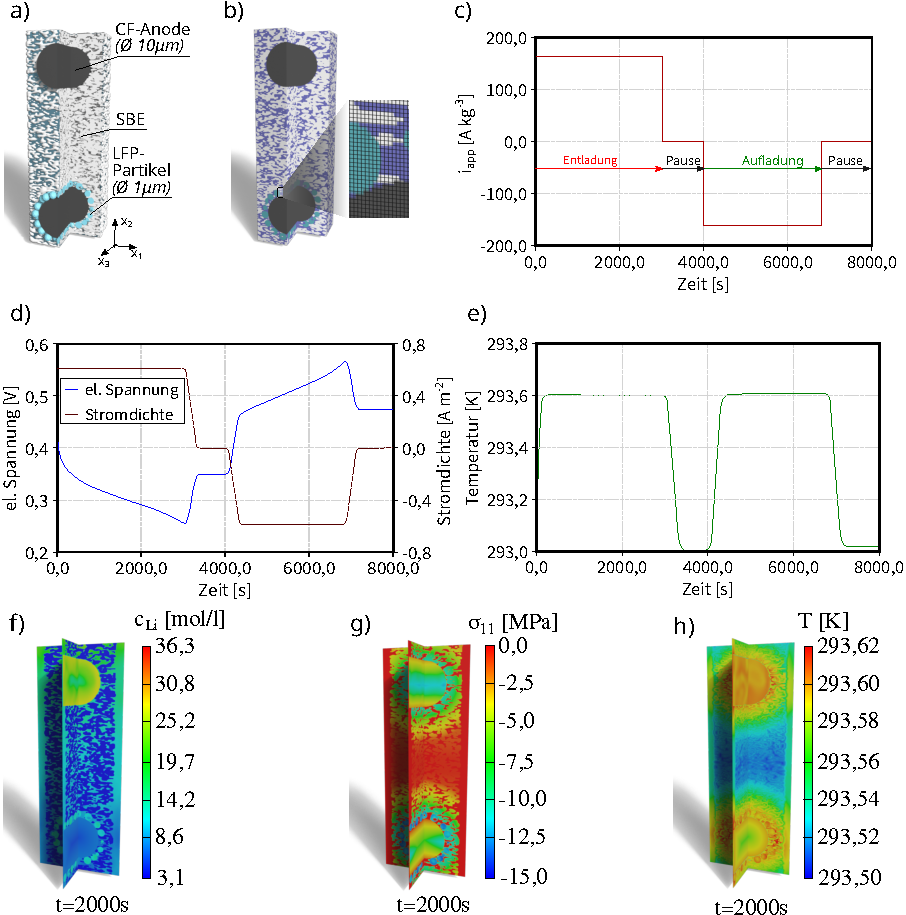
\includegraphics[width=0.8\textwidth, angle=0]{micro_model.pdf}
		\caption{\label{fig:micro_model}a) Eine Zwei-Faser-Batterie aus einer Kohlenstofffaser als Anode und einer mit LFP beschichten Kohlenstofffaser als Kathode. b) Blockvernetzung und Zuweisung der Domainen für die gekoppelte FE-Simulation c) Der angelegte Strom als treibende Randbedingung über die Zeit. d) Die elektrische Spannung und Stromdichte über die Zeit. e) Die gemittelte Temperatur über die Zeit. Die Lithiumkonzentration (f), die mechanische Spannung (g) und die die Temperaturverteilung (h) bei t = 2000s.}
\end{figure}

Die aus den Gleichungen folgende mikroskalige Simulation kann benutzt werden um Halbzellen mit Geometrien in ähnlichen Größenskalen zu simulieren~\cite{Plett2015}. Um ein Strukturbatteriezelle aus zwei Fasern korrekt zu simulieren, muss die allerdings auch die Struktur des zwei Phasenelektroltes entsprechend abgebildet werden\cite{Tu2020}. Die Geometrie basiert auf dem Prozess der Phasenseparierung, die mit der \textsc{Cahn-Hillard}-Gleichung modeliert werden kann\cite{Carolan2015,Grant1993}. 
\begin{align}
    \frac{\partial c}{\partial t} - \nabla \cdot M \left( \nabla \left( \frac{df}{dc} - \lambda \nabla^2 c\right) \right) &= 0 \text{ in }\Omega\\
    M\left( \nabla \left( \frac{df}{dc} - \lambda \nabla^2 c \right)\right) \cdot n &= 0 \text{ auf }\partial\Omega\\
    M \lambda \nabla c \cdot n &= 0 \text{ auf }\partial\Omega
\end{align}
Dabei wird die Separation der Konzentration der zwei Phasen $c$\footnote{Konznetrationswerte nahe -1 gehören zur ersten Phase, während Werte nahe 1 zur zweiten Phase zu geordnet werden.}, allein durch zwei Parameter $f$\footnote{Häufig eine in $c$ nicht-konvexe Polynomfunktion 4. Grades.} und $M$\footnote{Skalarer Wert} beschrieben. Da die \textsc{Cahn-Hillard}-Gleichung allerdings eine Gleichung 4. Ordnung ist fühert dies in der schwachen Formulierung zu Ortsableitungen zweiter Ordnung, was nicht mit Standard-Lagrange Elemente gelöst werden kann. Eine häufig verwendete Lösung für dieses Problem ist es die Gleichung durch Operationszerlegung umzuformulieren.
\begin{align}
    \frac{\partial c}{\partial t} - \nabla \cdot M \nabla \mu &= 0 \text{ in }\Omega\\
    \mu - \frac{\partial f}{\partial c} + \nabla^2 c &= 0 \text{ in }\Omega
\end{align}
Die Poren des resultierenden Strukturelektrolytes sind im Nanometerbereich. Allerdings liegen die LFP-Partikel und Kohlenstofffasern bei 1~$\mu m$ bzw. 10~$\mu m$. Daher wird ein sehr feines Netz benötigt\footnote{Im gezeigten Beispiel sind dies $180 \times 180 \times 640 = 20736000$ Elemente.}
Dies führt zusätzlich zu den nicht-linearen Differnetialgleichungen und den vielseitigen Kopplungen zu einem Berechnungsaufwand mehr als 2 Wochen um ein Ent- und Beladungs zu simulieren\footnote{Berechnungsserver der HTWK unter Ausnutzung von zwei eingebauten CPUs der Marke AMD EPYC 75F3 mit einer Taktrate von 2,95 Ghz und jeweils 32 Kernen} (Bild~\ref{fig:micro_model}). 




\section{\label{sec:homogenisation}Überführung der Mikroskaligen Modellierungsansätze in makroskalige Modelle durch Homogenisierung}

Die Modellierung der einzelnen phyiskalischen Prozesse sind oft einfacher auf der Mikroskale zu beschreiben~\cite{Plett2015}. Mit Hilfe dieser lassen sich Geometrie-, Verteilungs- und Clusterbildungseinflüsse ermitteln~\cite{Newman2021}. Jedoch ist der mit der hohen Komplexität durch die verschiedenen Skalenbereiche verbunde Berechnungsaufwand zu groß um mehrere Zellen damit zu simulieren~\cite{Liu2019}. Daher werden makroskalige Modelle benötigt, die den Berechnungsaufwand durch Homogenisierung und Modellvereinfachunngen reduziern~\cite{Plett2015}.

Ein häufig verwendeter Ansatz stellt dabei die Mittelung der physikalischen Eigenschaften über ein repräsentatives Volumenelement dar~\cite{Burow2016,Arunachalam2019,Li2020}. Die dazu mathematischen Grundlagen basieren auf drei Volumenmittlungstheoremen~\cite{Gray1977}.
\begin{enumerate}
    \item Volumenmittlung für ein skalares Feld $\psi$ 
    \begin{equation}
        \varepsilon_{\alpha} \overline{\nabla \psi_{\alpha}} = \nabla \left(\epsilon_{\alpha} \bar{\psi}_{\alpha} \right) + \frac{1}{V} \iint_{A_{\alpha \beta(\boldsymbol{x},t)}}\psi_{\alpha} \hat{\boldsymbol{n}}_{\alpha} \text{d}A
    \end{equation}
    \item Volumenmittlung für ein Vektorfeld $\boldsymbol{\psi}$
    \begin{equation}
        \varepsilon_{\alpha} \overline{\nabla \cdot \boldsymbol{\psi}_{\alpha}} = \nabla \cdot \left(\epsilon_{\alpha} \bar{\boldsymbol{\psi}}_{\alpha} \right) + \frac{1}{V} \iint_{A_{\alpha \beta(\boldsymbol{x},t)}}\boldsymbol{\psi}_{\alpha} \cdot \hat{\boldsymbol{n}}_{\alpha} \text{d}A
    \end{equation}
    \item Volumenmittlung für die zeitliche Änderung eines skalaren Feldes $\psi$ 
    \begin{equation}
        \varepsilon_{\alpha} \overline{\left[\frac{\partial \psi_{\alpha}}{\partial t}\right]} = \frac{\partial \left(\epsilon_{\alpha} \bar{\psi}_{\alpha} \right)}{\partial t} - \frac{1}{V} \iint_{A_{\alpha \beta(\boldsymbol{x},t)}}\psi_{\alpha} \boldsymbol{v}_{\alpha \beta} \cdot \hat{\boldsymbol{n}}_{\alpha} \text{d}A
    \end{equation}
\end{enumerate}
Dabei beschreibt $\bar{\psi}_{\alpha}$ bzw. $\bar{\boldsymbol{\psi}}_{\alpha}$ die intrinsischen Mittelung über Phase $\alpha$. Diese Art der Mittelung wird nur über das von Phase $\alpha$ eingenommene Volumen\footnote{Hier als zwei Phasensystem mit der zweiten Phase $\beta$ betrachtet.} ermittelt. Die intrinische Mittelung erlaubt gegenüber einer klassischen Mittelung $\langle \psi_{\alpha} \rangle$, welcher auf das Volumen des gesamten Gebietes bezogen ist, eine größere Flexibilität und wieder Verwendbarkeit. Mittels des Volumenanteils $\varepsilon_{\alpha}$
\begin{equation}
    \varepsilon_{\alpha} = \frac{V_{\alpha}(\boldsymbol{x},t)}{V} 
\end{equation}
können die beiden Mittelungsarten in einander umgewandelt werden.
\begin{equation}
    \langle \psi_{\alpha} \rangle = \varepsilon_{\alpha} \bar{\psi}_{\alpha}
\end{equation}

Mit Hilfe der drei Volumenmittelungstheoreme lassen sich die folgenden vier Gleichungen herleiten~\cite{Doyle1995}.
\begin{enumerate}
    \item Volumengemittelte Annäherung des Ladungserhaltes in der festen Phase der porösen Elektrode
    \begin{equation}
        \nabla \cdot \left(\sigma_{\text{eff}} \nabla \hat{\phi}_{s} \right) = a_s F_{\text{K}} \hat{j}
    \end{equation}
    \item Volumengemittelte Annäherung des Ladungserhaltes in der Elektrolytphase der porösen Elektrode
    \begin{equation}
        \nabla \cdot \left(\kappa_{\text{eff}} \nabla \hat{\phi}_e + \kappa_{D, \text{eff}} \nabla ln \hat{c}_e\right) + a_s F_{\text{K}} \hat{j} = 0
    \end{equation}
    \item Volumengemittelte Annäherung des Massenerhaltes in der Elektrolytphase der porösen Elektrode
    \begin{equation}
        \frac{\partial \left(\varepsilon_e \hat{c}_e \right)}{\partial t} = \nabla \cdot \left(D_{e,\text{eff}}\nabla\hat{c}_e\right) + a_s (1+t^0_+) \hat{j}
    \end{equation}
    \item Volumengemittelte Annäherung der mikroskopischen Butler-Volmer Beziehung für den Ionenphasenwechsel
    \begin{equation}
        \hat{j} = j(c_{s,e},\hat{c}_e,\hat{\phi}_s,\hat{\phi}_e)
    \end{equation}
\end{enumerate}

Analog lassen sich für die mechansiche Spannung und die Temparatur die folgenden Zusammenhänge aufstellen.
\begin{enumerate}
    \item Homogenisierung der mechansichen Spannung
    \begin{equation}
    \boldsymbol{\sigma} = \boldsymbol{C}_{\text{eff}} \boldsymbol{\varepsilon}_{\text{mech}} 
    \end{equation}
    \item Volumengemittelte Annäherung der Temperatur
    \begin{equation}
        \frac{\partial (\rho c_{\text{P}} T)}{\partial t} = \nabla \cdot (\lambda \nabla T) + q
    \end{equation}
\end{enumerate}
Der neu eingeführte Wärmegenerierungsterm $q$ kann dabei aus den folgenden fünf Quellen zusammengesetz werden~\cite{Plett2015}.
\begin{enumerate}
    \item Irreversible Wärmeentstehung durch chemische Reaktionen\footnote{Für jede chemische Reaktion $j$.}
    \begin{equation}
        q_i = a_{\text{s}} F_{\text{K}} \hat{j}_j \eta_{j}
    \end{equation}
    \item Rreversible Wärmebildung durch Verädnerung der Entropie\footnote{Für jede chemische Reaktion $j$.}
    \begin{equation}
    q_{r} = a_{\text{s}} F_{\text{K}} \hat{j}_j \eta_{j} T \frac{\partial U_{\text{ocp},j}}{\partial T}
    \end{equation}
    \item Joule-Wärmeentstehung durch Gradient des elektrischen Potenzials im Feststoff
    \begin{equation}
    q_{s} = \sigma_{\text{eff}}(\nabla\hat{\phi}_{\text{s}} \cdot \nabla\hat{\phi}_{\text{s}})
    \end{equation}
    \item Joule-Warmeentstehung durch Gradient des elektrischen Potenzials im Elektrolyt
    \begin{equation}
        q_{e} = \kappa_{\text{eff}}(\nabla\hat{\phi}_{\text{e}} \cdot \nabla\hat{\phi}_{\text{e}}) + \kappa_{D,\text{eff}} (\nabla ln \hat{c}_e \cdot \nabla \hat{\phi}_{\text{e}})
    \end{equation}
    \item Warmeentstehung durch Kontaktwiderstände\footnote{$q_c$ gilt nur für die Elektodenfläche und ist daher bezogen auf die Einheitsfläche und nicht wie die anderen Therme auf das Einheitsvolumen}
    \begin{equation}
        q_{c} = i_{\text{app}}^2 R_{\text{Kontakt}}
    \end{equation}
\end{enumerate}

\begin{figure}[!h]
	%\raggedleft
		%\def\svgwidth{\columnwidth}
        \center
		\includegraphics[width=0.8\textwidth, angle=0]{carlstedt.pdf}
		\caption{\label{fig:carlstedt}a) Schematische Darstellung der zu analysierenden Kohlenstofffaser-Strukturbatterie und LFP Zelle angelehnt an Studien von \textsc{Carlstedt}~\cite{Carlstedt2022b}. b) 2D-Model für die FEM Berechnung. c) Der angelegte Strom als treibende Randbedingung über die Zeit. d) Die elektrische Spannung und Stromdichte über die Zeit und die Lithiumkonzentration an den beiden Zeitpunkten $t_1= 2000s$ und $t_2= 6000s$. e) Die gemittelte Temperatur über die Zeit und die Temperaturverteilung bei $t_1$ und $t_2$. f) Die mechanischen Spannungskomponenten $\sigma_{11}$ und $\sigma_{22}$ zu $t_1$ und $t_2$.}
\end{figure}

Angelehnt an Arbeiten von \textsc{Carlstedt}~\cite{Carlstedt2022b}\footnote{Die Materialwerte und Geometrie, sowie die Randbedingung wurden aus der Arbeit entnommen um einen Vergleich zu haben.} können diese Gleichungen bereits benutzt werden, um das Verhalten  ganzer Zellen zu beschreiben\footnote{Hier eine Kohlenstofffaser-LFP-Zelle} (Bild~\ref{fig:carlstedt}). Die Zelle durch läuft dabei einen Entladungs- und Ladezyklus innerhalb von 2,2 h. Die Simulationszeit betrug dabei 34,6 h auf einem Berechnungsserver der HTWK\footnote{Unter voller Ausnutzung von zwei eingebauten CPUs der Marke AMD EPYC 75F3 mit einer Taktrate von 2,95 Ghz und jeweils 32 Kernen}. Der hohe Berechnungsaufwand für breits einen Ladezyklus macht diesen Ansatz jedoch ungeeignet um eine Vielzahl an Varianten und größere, mehrzellige Batteriesysteme vorauszulegen.

Um die Berechnugnszeit weiter zu reduzieren, kann zwar wegen der Butler-Volmer Randbedingung keine Volumenmittelung für die Massenerhaltung in der festen Phase\footnote{Die Materialien, die als Interkalationsort dienen} benutzt werden~\cite{Plett2015}, jedoch können durch Geometrievereinfachungen Freiheitsgrade reduziert werden und zusätzlicher Berechnungsaufwand vermieden werden. Im Kontext von Strukturbatterien ist der an der Interkalation aktiv teilnehmende Teil Partikel- oder Faserförmig, welche durch Kugeln oder Zylinder approximiert werden könnent~\cite{Newman2021}.
\begin{enumerate}
    \item Spezialfall Massenserhalt in kugelförmigen Festkörpern
    \begin{equation}
    \frac{\partial c_{\text{s}}}{\partial t} = \frac{1}{r^2} \frac{\partial}{ \partial r} \left[ D_{\text{s}} r^2 \frac{\partial c_{\text{s}}}{\partial r}\right]
    \end{equation}
    \item Spezialfall Massenserhalt in zylindrischen Festkörpern
    \begin{equation}
    \frac{\partial c_{\text{s}}^{\pm}}{\partial t} = \frac{1}{r} \frac{\partial}{ \partial r} \left[ D_{\text{s}} r \frac{\partial c_{\text{s}}}{\partial r}\right] + \frac{\partial}{ \partial z}\left[D_{\text{s}}  \frac{\partial c_{\text{s}}}{\partial z}\right]
    \end{equation}
\end{enumerate}
In beiden Fällen lässt sich das Interkalationsverhalten durch die beiden Randbedingungen
\begin{align}
    \left.\frac{\partial c_{\text{s}}^{\pm}}{\partial r}\right\vert_{r=0} &= 0 \\
    \left.\frac{\partial c_{\text{s}}^{\pm}}{\partial r}\right\vert_{r=R_{\text{p,s}}^{\pm}} &= -\frac{1}{ D_{\text{s}}^\pm} j_{n}^{\pm}(x,t)
\end{align}
dargestellt, wobei im Falle einer Stromgesteuerten Be- und Entladung
\begin{equation}
j_{n}^{\pm}(t) = \mp \frac{I(t)}{F a^{\pm} L^{\pm}}
\end{equation}
ist.

Durch ermittlung effektiver physikalischer Eigenschaften werden dabei die Inhomognitäten auf der Mikroskale durch ein Kontinuum auf der Markoskale beschrieben~\cite{Plett2024}. Die Genauigkeit dieses Ansatz hängt jedoch stark von dem zu betrachten Dimensionen ab~\cite{Plett2015}. Durch die Beschreibung als Kontinuum können Einglüsse wie etwa eine lokal höhere Porendichte nur aufwendig berücksichtigt werden~\cite{Mei2019}. Bei der Analyse von deutlich größeren Skalen, als die Inhomogenität, zeigen diese Modelle dafür eine hohe Genauigkeit~\cite{Plett2015}. 



\begin{figure}[!h]
	%\raggedleft
		%\def\svgwidth{\columnwidth}
        \center
		\includegraphics[width=0.5\textwidth, angle=0]{simulation_model.pdf}
		\caption{\label{fig:homogenisation}Mehrskalige Homogenisierung der Strukturbatterie durch Abstraktion der Geometrie, }
\end{figure}

\begin{figure}[!h]
	%\raggedleft
		%\def\svgwidth{\columnwidth}
        \center
		\includegraphics[width=0.5\textwidth, angle=0]{bending.pdf}
		\caption{\label{fig:bending}Validierung des 3-Punkt-Biegefalls durch: a) Visueller Vergleich von Simulation und Experiment und b) Kraftverlauf in Abhängigkeit der Durchbiegung für Pouchzellen mit und ohne Elektrolyt.}
\end{figure}



\chapter{Entwicklung einer hybriden Auslegung von Strukturbatterien}
Die Modelle, die sich aus den Arbeiten von \textsc{Carlstedt}, \textsc{Doyle}, \textsc{Newman}, \textsc{Fuller} und \textsc{Plett} ergeben sind mit einem hohen hohen Detailgrad versehen. Dieser Detailgrad erlaubt eine hohe physikalische Präzesion, jedoch sorgt dies gleichzeitig für eine hohe Anzahl an Parametern, die aufwenig bestimmt werden müssen. Damit entsteht das Problem, dass in bestimmten Konstellationen es schneller und günstiger ist direkt Experimente mit allen Materialkombinationen zu machen, als erst alle benötigten Material- und Interaktionsparamter zu bestimmen. Um dies einzuschätzen und eine möglichst optimale Entwicklungsstrategie wird in Kapitel~\ref{sec:efficent_development} ein entsprechendes Auswahl und Bewertungsrahmenwerk entwickelt. Mit Hilfe dieses werden in den Kapiteln~\ref{sec:improve_elchem} und \ref{sec:improve_mech} eine Reihe an häufig gültigen Vereinfachungen der elektrochemische und mechansichen Modellierung unternommen. Um die Einsatzfähigkeiten der verschiedenen Strukturbatterie automatisiert bewerten zu können wird in Kaptiel~\ref{sec:automated_failure} ein Versagens- und Risikoabschätzung vorgestellt. Abschließend wird in Kapitel~\ref{sec:digitalisation} auf die Umsetzung der digitalen und automatisierten Vorauswahl geegineter Strukturbatteriekonfigurationen eingegangen.

\section{\label{sec:efficent_development}Konzeptionierung eines effizienten Entwicklung von Strukturbatterien}
Für den effektiven Einsatz der Modellen für die Vorhersage von mechansichen und elektroschmeischen Eigenschaften wurde eine Vielzahl an Anforderungen an die Modellierung gesammelt:
\begin{itemize}
    \item Moddelierung baiserend auf physikalischen Prozessen, % kein Fitting
    \item geringe Materialparameteranzahl und keine Einführung Neuer, % aufwendige bestimmung
    \item präzise genug für Vergleichbarkeit zwischen mehreren Ergebnissen, % 
    \item schnelle Berechnungen. % nicht wochenlang rechnen
\end{itemize} 

Diese Anforderungen folgen aus der Annahme, dass experimentell erworbene Ergebnisse das reale Verhalten des Objektes unter Beobachtung darstellen. Aus dieser Annhame folgt, dass sich simulative Ergbenisse maximal den experimentellen Ergebnissen annähern und damit folglich stehts ungenauer sind, solange experimentelle Messfehler vernachlässigt werden können~\cite{Morris2024}. Jedoch ist mit diesen hochwerigen Experimenten verbunde Aufwand ($k_{\mathrm{exp}}$) hinsichtlich Material-  und Zeitkosten oftmals um einiges höher als der Aufwand die Simulation mithilfe eines Computers zu berechnen ($k_{\mathrm{sim}}$).
\begin{equation}
    k_{\mathrm{exp}} \ll k_{\mathrm{sim}} 
\end{equation}
Für einen rein experimentellen Ansatz der jede mögliche Materialkombination ($n_{\mathrm{Kombis}}$) einer bestimmten Anzahl an experimentellen Bestimmungen ($n_{\mathrm{exp,Bestimmungen}}$) unterzieht ergibt sich der gesamte Aufwand ($k_{\mathrm{exp, gesamt}}$) wie folgend.
\begin{equation}
    k_{\mathrm{exp, gesamt}} = k_{\mathrm{exp}} \cdot n_{\mathrm{Kombis}} \cdot n_{\mathrm{exp,Bestimmungen}}
\end{equation}
Wie 
Um wie im konkreten Beispiel knapp 1000 verschiedene Kombination zu testen sind Modelle also unablässig. Dennoch muss sich auch der Auffwand der Modellierungstrategie ($k_{\mathrm{sim, gesamt}}$) in Grenzen halten, da sich der Modellierungsaufwand aus der Summe der für Materialparameter notwenigen Untersuchungen und dem Berechnungsaufwand ergibt.
\begin{align}
    k_{\mathrm{sim, gesamt}} &= k_{\mathrm{sim}} \cdot n_{\mathrm{Kombis}} \cdot n_{Rechnungen} \nonumber \\
    &+ \sum_{m}^{n_{\mathrm{Material}}} n_{\mathrm{exp, Bestimmung}} \cdot k_{\mathrm{exp}} + n_{\mathrm{lit, Bestimmung}} \cdot k_{\mathrm{lit}} 
\end{align}
Da wie bereits am Anfang beschrieben Modelle sich maximal der Präzesion durch Experimente annähern, ist es unter Berücksichtigungen der verschiedenen Aufwände naheliegend mittels der Modellierungsmethodik soviele wie mögliche Materialkandidaten herauszufiltern und im Anschluss diese besten Kombination mittels Experimente zu identifizieren.


\section{\label{sec:improve_elchem}Identifizierung elektrochemischer Materialparameter}

Das hergeleitet Modell zur multi-physikalischen Beschreibung der Strukturbatterie auf der Mikroskala benötigt in der kompletten ausführung 18 zu bestimmende Parameter für jede faserbasierte Elektrode, 11 Parameter pro Elektrolytesystem und faserbasierten Separato, und zwei Interaktionskoeffizienten für jede Kombination an Elektrode und Elektrolyte. Hinzukommen 10 Parameter die für transversal Isotropematerialien, die als Pouchbag und damit nicht an der Reaktion teilnehmen.


\begin{itemize}
    \item Diffusionskoeffizient wird durch equivalente Schaltung ermittelt, die konstanten Wert vorraussetzen
    \item Diffusionskoeeffizeint ist eigentlich stark von der Lithierung abhängig
    \item aufwendig zu ermitteln
    \item außerdem abweichungen durch Bildung Elektrolyteinterface
    \item daher für vorhersagen ist die benutzung eher ungeeignet
    \item für Batterien ist Energidichte wichtiger als Leisungsdichte
    \item Lösung quasistatische Be- und Entladung, also warten bis vorher
    \item dies reduziert die vereinfacht die oberen Gleichungen enorm
\end{itemize}

\begin{equation}
    C_{\text{A, Zelle}} = \min \left( C_{\text{A, -}} , C_{\text{A, +}}\right)
\end{equation}

\begin{equation}
    C_{\text{A, Stack}} = n_{\text{Zellen}} \cdot C_{\text{A, Zelle}}
\end{equation}

\begin{equation}
    m_{\text{A, Stack, E}} = C_{\text{A, Stack}} \cdot V_{\text{C,E}} \cdot \rho_{\text{E}}
\end{equation}

\begin{equation}
    m_{\text{A, Stack}} = m_{\text{A, Stack, E}} + \sum_{i}^{n_{\text{Schichten}}} m_{\text{A,i}} 
\end{equation}

\begin{equation}
    C_{\text{m, Stack}} = \frac{C_{\text{A, Stack}} }{ m_{\text{A, Stack}}}
\end{equation}

\begin{equation}
    \Gamma_{\text{Stack}} = C_{\text{m, Stack}} \cdot \left(U_{+} - U_{-}\right)
\end{equation}

% aus: Simultaneously Coupled
% Mechanical-Electrochemical-
% Thermal Simulation of Lithium-
% Ion Cells
\begin{align}
    R_{\text{Kurz}} &= A_{\text{Kurz}} \sum_{i} \frac{1}{K_i}\\
    A &= \sum_{i}^{n_{\text{Versagen}}} A_{i}
\end{align}

\begin{equation}
    V_{\text{Zelle}} = (U_{+} - U_{-} + \sum_{j=+,-} \frac{2 RT}{F} ln\left(\frac{\sqrt{m_j^2 +4} + m_j}{2}\right) - i_{app} R_{\text{Kurz}}
    m_j = \frac{i_{app}}{F k_j S_j c_{s,j}^{max} \sqrt{c_e (1-x_{Li,j}) x_{Li,j}}} 
\end{equation}

\begin{equation}
    \rho v c_p \frac{\partial T}{\partial t} = i_{app}\left(V_{\text{Zelle}} - U_{+} + U_{-} + i_{app} R_{Kurz} \right) -q
\end{equation}

\begin{equation}
    q = 0
\end{equation}

\section{\label{sec:improve_mech}Identifizierung mechanischer Materialparameter}
Unter der Annahme, dass alle Einzelschichten bei der Bestimmung der Zugsteifigkeit auf beiden Seiten in der Klemmung mit aufgenommen werden und keiner Vordehnung der Einzelschichten sind die Dehnungen in Zugrichtungen für alle Schichten gleich.
\begin{equation}
    \varepsilon_{x,ges} = \varepsilon_{x,i}\\
\end{equation}



\subsection*{Reduktion des Berechnungsaufwandes für 3-Punkt-Biegebelastungen unter Berücksichtigung verschiederner Elektrolytarten}

Der Struktur von konventionellen Batterien oder Strukturbatterie mit Gel oder flüssigem Elektrolytsystemen kann vereinfacht als Schichtung, lastentragende Materialien betrachtet werden, in deren Zwischnraum eine nicht-lastentragenden Substanz in Form eines Flüssigen oder Gelartigen Zustandes infiltriert wurde.
Die einzelnen Schichten sind nicht direkt mit einander verbundnen und halten einzig durch den Druck der durch die äußere Pouchfolie aneinander. Unter der Annahme, dass die Sichten sich lückenlos anschmiegen ist davon aus zugehen, dass die Krümmung $\kappa$ mit
\begin{equation}
    \kappa = \frac{1}{r} = \frac{M_y}{E I_y}
\end{equation}
in jeder Schicht gleichgroßt ist.
\begin{equation}
    \kappa = \kappa_1 = \kappa_2 = \dots = \kappa_i = \dots = \kappa_n
\end{equation}
Des Weiteren folgt aus dem Momentengleichgewicht, dass das außen angreifende Biegemoment $M_{b}$ gleich der Summe der Schnittmomente in den Einzelschichten sein muss.
\begin{equation}
    M_{b} = \sum_{i}^{n}M_{y,i}
\end{equation}
Unter Annahme von rechticken Querschnitten mit Breite $b_i$ und Höhe $h_i$ und der Annhame, dass alle Elektroden näherungsweise gleich Breit sind, also $b_i = b$ gilt, folgt für die Belastung einer Einzelschicht durch das Moment $M_i$:
\begin{align}
    M_{b} &= M_i \sum_{k}^{n}\frac{E_k I_{yy,k}}{E_i I_{yy,i}}\\
    M_{b} &= M_i \frac{\sum_{k}^{n} E_k h_k^3}{E_i h_i^3}\\
    M_i &= M_{b} \frac{ E_i h_i^3} { \sum_{k}^{n}E_k h_k^3}
\end{align}
Durch einsetzen Einzelschichtbelastung in die Formel zur Bestimmung der Biegespannung erhält man einen Zusammenhang zwischen Einzelschichtspannung und Biegemomentenbelastung:
\begin{align}
    \sigma_{b,i} &= \frac{M_y,i}{I_{yy}/h_i} \\
    \sigma_{b,i} &= 12 \frac{ M_y,i}{b h_i^2}\\
    \sigma_{b,i} &= 12 \frac{M_{b} E_i h_i^3}{b h_i^2 \sum_{k}^{n}E_k h_k^3}\\
    \sigma_{b,i} &= 12 \frac{M_{b} E_i h_i}{b \sum_{k}^{n}E_k h_k^3}
\end{align}

Für die Bestimmung der Durchbiegung $u$ beim 3-Punkt-Biegeversuch kann 
unter der
\begin{equation}
\frac{\frac{\partial^2 u(x)}{\partial x^2}}{\left(1 + \left(\frac{\partial u(x)}{\partial x} \right)^2 \right)^{3/2}} = -\frac{M_y}{E I_{yy}}
\end{equation}
Diese Gleichung kann für kleine Verformungen, so dass $(\frac{\partial u(x)}{\partial x})^2 \ll 1$ durch die folgende Näherung ersetzt werden.
\begin{equation}
    \frac{\partial^2 u(x)}{\partial x^2} \approx -\frac{M_y(x)}{E I_{yy}}
\end{equation}

Unter der Annhame kleiner Verformung und konstantem Querschnitt und Steifigkeit lässt sich die Durchbiegung infolge der Kraft F durch folgende Gleichung annähern.
\begin{align}
    u(x) &= \frac{F L^3}{48 \sum_{k}^{n} E_k I_{yy,k}} \left[ 3 \frac{x}{L} - 4\left(\frac{x}{L}\right)^3 \right] \text{für} \; 0 \leq x \leq L/2 \\
    u_{max} (x = L/2) &= \frac{FL^3}{48 \sum_{k}^{n} E_k I_{yy,k}} 
\end{align}



An dieser Stelle ist zu bemerken, dass für Spezialfall wo alle $n$ Schichten gleich dick sind und aus dem gleichen Material bestehen, die Spannung sich wie folgend ergibt.
\begin{equation}
    \sigma = \sigma_i = \frac{12 M_{b}}{n b h^2},
\end{equation}
Diese Formel ist bereits im Kontext geschichteter Blattfedern bekannt und ist, was 

Druchbiegung $u_max$
\begin{equation}
    u_{max} = \frac{L^3 Q}{4 n b h^3 E} = \frac{L^2 \sigma}{6 h E}
\end{equation}
ergibt sich die 


Im Verhältniss zum stofflichen Verbund ist davon auszugehen, dass diese Steifigkeitssteigerung deutlich geringer ist, wenn aber auch nicht komplett vernachlässigbar.


\section{\label{sec:automated_failure}Automatisierte Versagensanalyse für Strukturbatterien und Risikoeinschätzung}

Mit Hilfe der entwickelten Modelle, kann der Spannungszustand $\boldsymbol{\sigma}$ in den einzelnen Materialien innerhalb der Strukturbatterie bestimmt werden. Durch geeignet Versagenskriterien kann ein mechanisches Versagen der Schichten ermittelt werden.  
Typsiche Versagenskriterein für isotrope 


\begin{table}[ht]
    \centering
    \caption{\label{tab:failure_modes}Überischt des mit Versagens der Einzelschichten verknüpften Sichheitsrisikos.}
    \begin{tabularx}{\textwidth}{lXXX}
    \toprule
    &\makecell{Pouchfolienversagen\\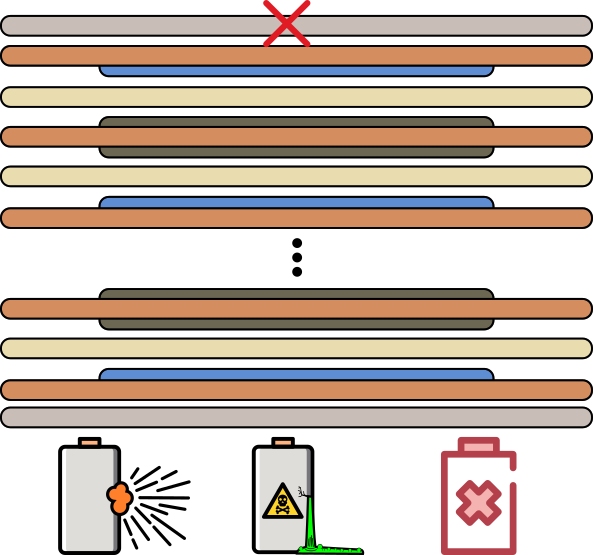
\includegraphics[width=0.2\textwidth]{failure_modes/failure_mode_pouch.png}}
    &\makecell{Elektrodenversagen\\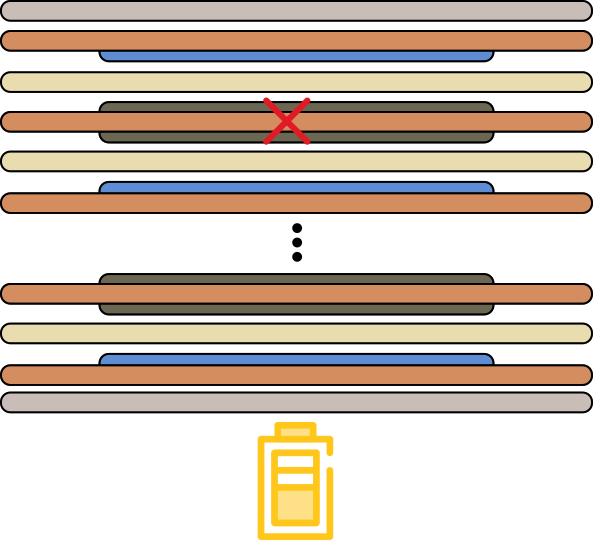
\includegraphics[width=0.2\textwidth]{failure_modes/failure_mode_electrode.png}}
    &\makecell{Separatorversagen\\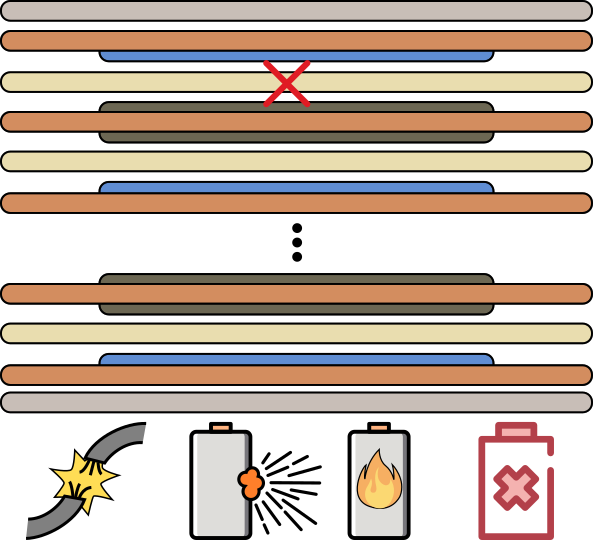
\includegraphics[width=0.2\textwidth]{failure_modes/failure_mode_separator.png}}
    \\
    \midrule
    Funktion
        & Funktionsversagen der gesamten Batterie durch austrocknen
        & Leistungsverlust der Zelle
        & Funktionsversagen der Zelle, je nach Verschaltung auch der gesamten Batterie
    \\
    Brandgefahr
        & kein Risiko
        & kein Risiko
        & Flammenbildung durch Überhitzung
    \\
    Gesundheit
        & hohes Risiko durch austretendes Elektrolyt
        & kein Risiko
        & kein zusätzliches Risiko
    \\
    \bottomrule
    \end{tabularx}\\
    %\noindent{\footnotesize{\textsuperscript{*} Gemessen gegenüber \ce{Li}/\ce{Li+}.}}
\end{table}%

\section{\label{sec:digitalisation}Erstellung einer Materialdatenbank für Strukturbatterien}